\documentclass[12pt]{article}
\usepackage{enumitem}
\usepackage{graphicx}
\begin {document}

	\large \textbf{A Proposed Implementation of an 8 Bit ALU Bit Slice}
	\normalsize
	\begin{center}
		Arjun Lakshmipathy, ID: 804158733 \\
		Joraaver Chahal, ID: 304200975
	\end{center}
  \section{}

	\textbf{High Level Description:}
	\newline \newline
	Our decided implementation of the bit slice for this 8 bit ALU attempted to target
	minimizing the energy delay product while keeping the overall design as intuitive and 
	readable as possible. Our decided upon implementation was a reasonably modular 
	slice comprised of a combination of simpler gates with varying numbers of inputs. Our
	solution to minimizing the energy product delay of the whole slice was to limit the number
	or transistors used in the circuit. However, in some cases extra transistors were added
	simply to either:
	
	\begin{enumerate}[label=(\alph*)]
		\item Keep the design more readable / maintainable. 
		\newline \newline
		or
		\item Allow a particular component of the circuit to be self-restoring. 
	\end{enumerate}
	These tradeoffs were determined as acceptable since they would simplify some of the
	development process moving forward and would ensure that we did not experience any
	unexpected signal degradation. 
	\newline \newline
	Using this approach, we began constructing some basic gates at the transistor level. The most
	basic gates constructed were the following:
	\begin{itemize}
		\item Inverter
		\item 2-input NAND
		\item 3-input NAND
		\item 2-input NOR
		\item 3-input XOR
		\item Transmission Gate
		\item 2-input MUX
		\item 8-input MUX
		\item 2-output DEMUX
	\end{itemize}
	All other components of the circuit were more or less assembled from these basic building
	blocks. These included:
	\begin{itemize}
		\item 2-input AND
		\item 3-input AND
		\item 2-input OR
		\item Logical Shift (left or right)
		\item Adder
	\end{itemize}
	Finally, using these higher level building blocks, we constructed the "Master" high level
	schematic to serve as our control for the overall slice.Using our master schematic as 
	the control and the components as the actual operations of the ALU, we constructed 
	our overall single bit slice. 
	\newline \newline
	\textbf{More Detailed Breakdowns:}
	\newline \newline
	\textbf{OR-NOR-AND etc. Implementation and Uses:}
	\newline \newline
	Each of these gates was constructed using a static CMOS layout, with the PMOS pull-up 
	network being complementary to the NMOS pull-down network. Each gate was driven by
	its own voltage supply and was connected to ground to ensure that it could drive itself and
	not be dependent on the input. Some of these gates were used as final outputs of the ALU,
	while others were used to build more complex modules or serve as control blocks. The 
	transistors were sized such that both the pull-up and the pull-down network
	both resulted in an ultimate unity resistance, using a base unit of 3$\lambda$. 
	For reference, see some samples below:
	\newline \newline \newline \newline \newline \newline \newline
 	3-input and:\\
  	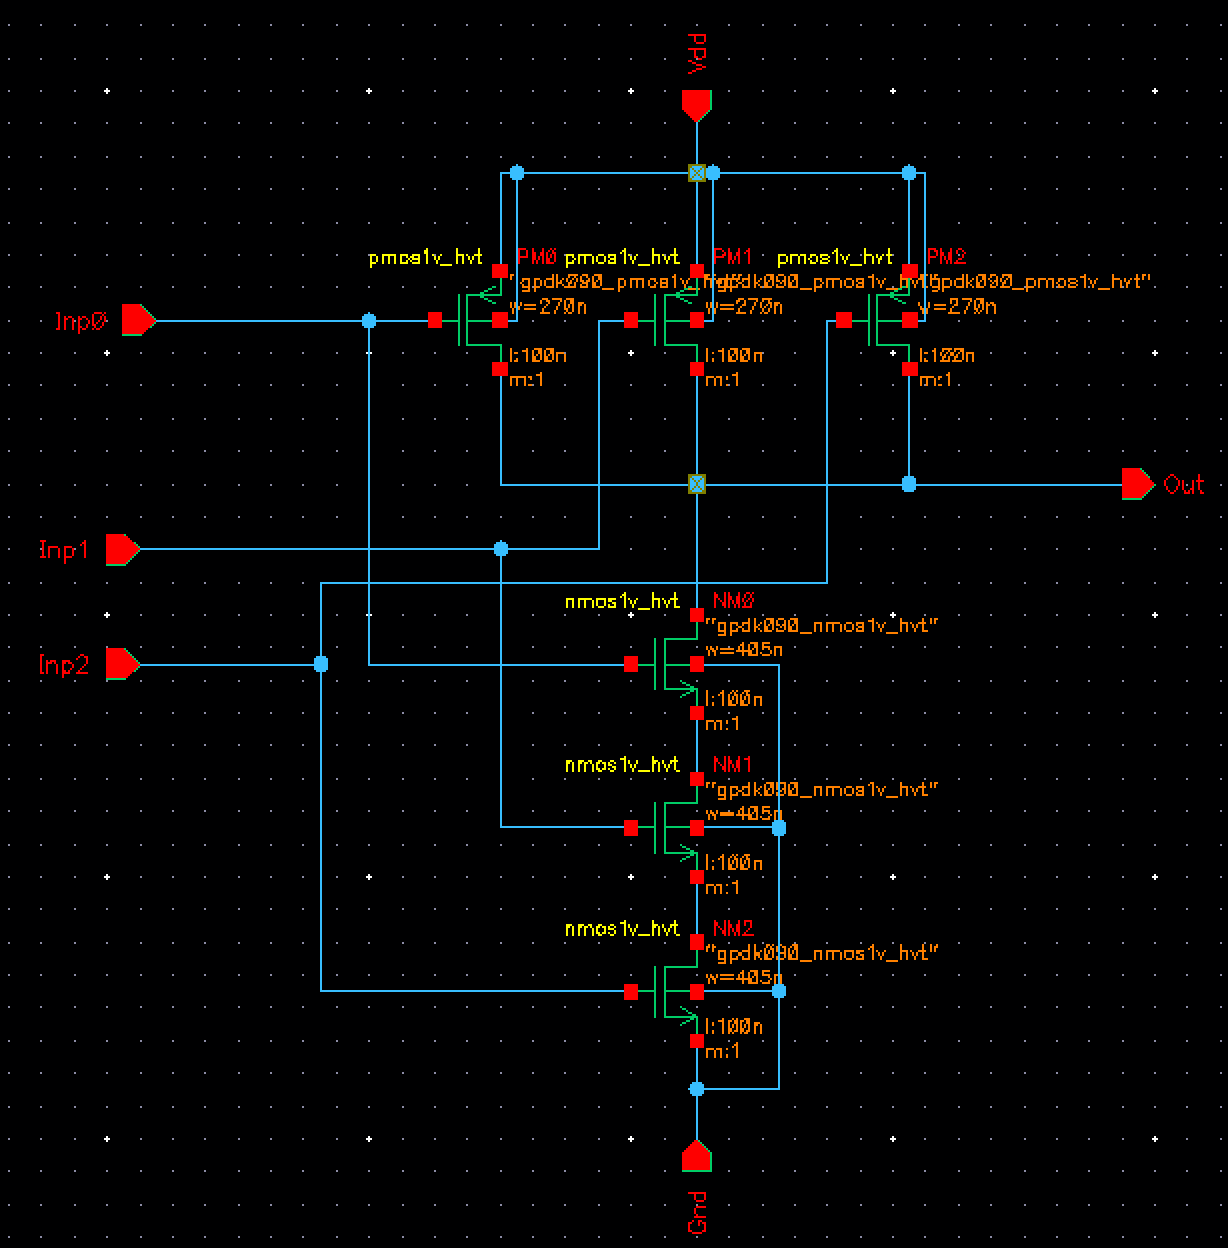
\includegraphics[scale=0.4]{3and.png} \\
	\newline \newline
  	3-input xor:\\
 	 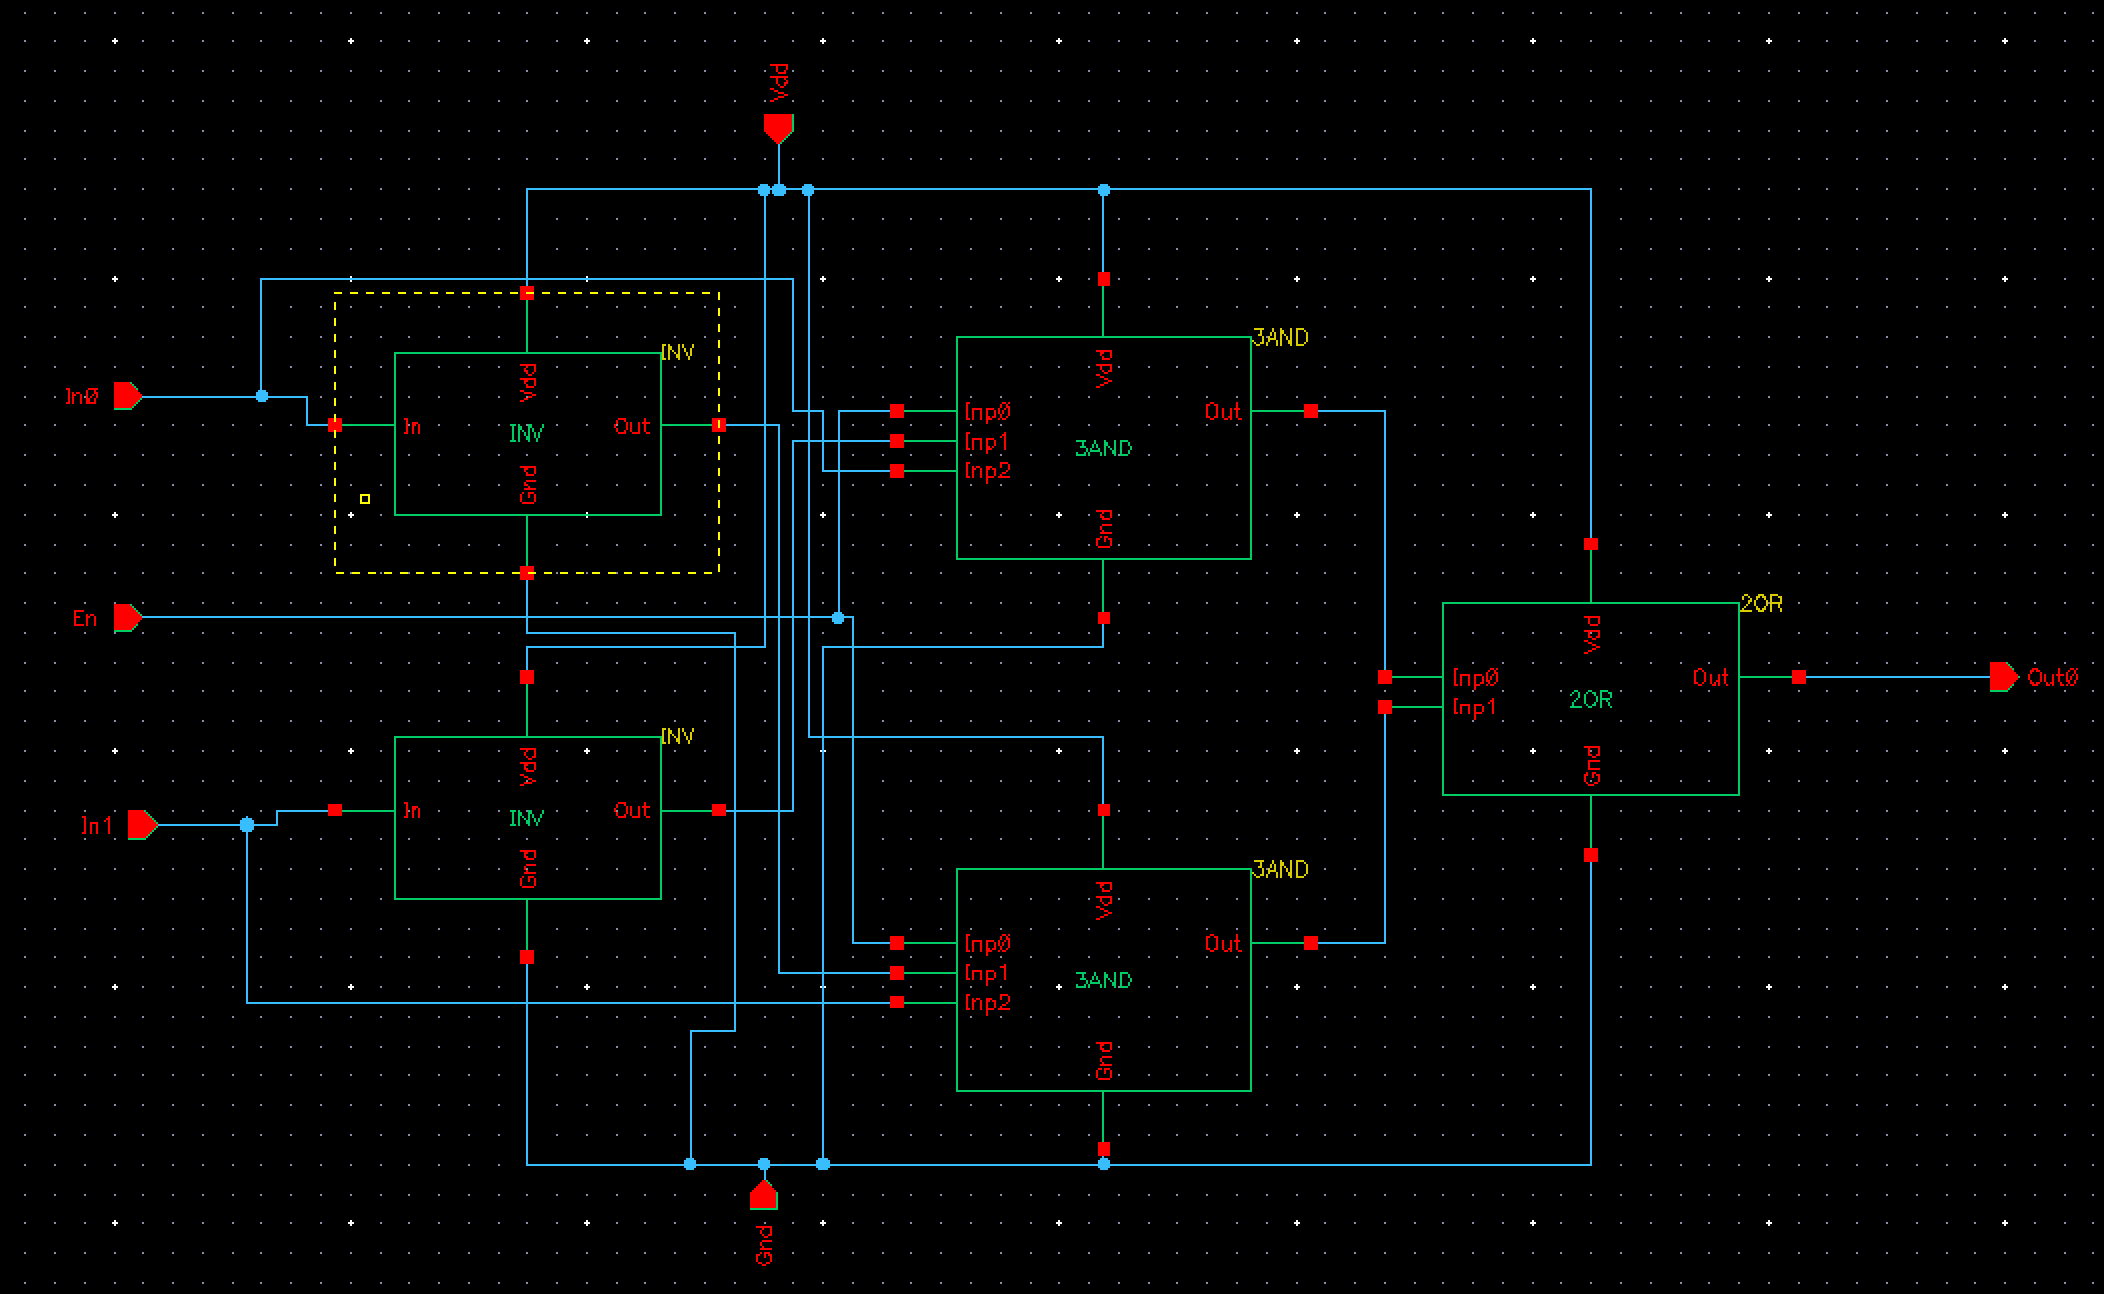
\includegraphics[scale=0.3]{xor.png} \\
	\newline \newline
	\textbf{MUX / DEMUX Implementation and Uses:}
	\newline \newline
	The primary building blocks for each of these gates were transmission gates, with each 
	T-Gate having a 3$\lambda$ NMOS and a 6$\lambda$ PMOS. These gates primarily served
	as control logic for the circuit (our master schematic heavily relies on DEMUX gates), 
	allowing us to handle multiple input modules and granting us the ability to selectively 
	activate only certain portions of the ALU during any particular OpCode
	in order to minimize power consumption. They also served very crucial roles in allowing us to
	compress the left and right shift modules into one by cleverly mapping the input and easily 
	implement the clear operation. The implementation of these gates are pictured below:
	\newline \newline
 	Transmission gate:\\
 	 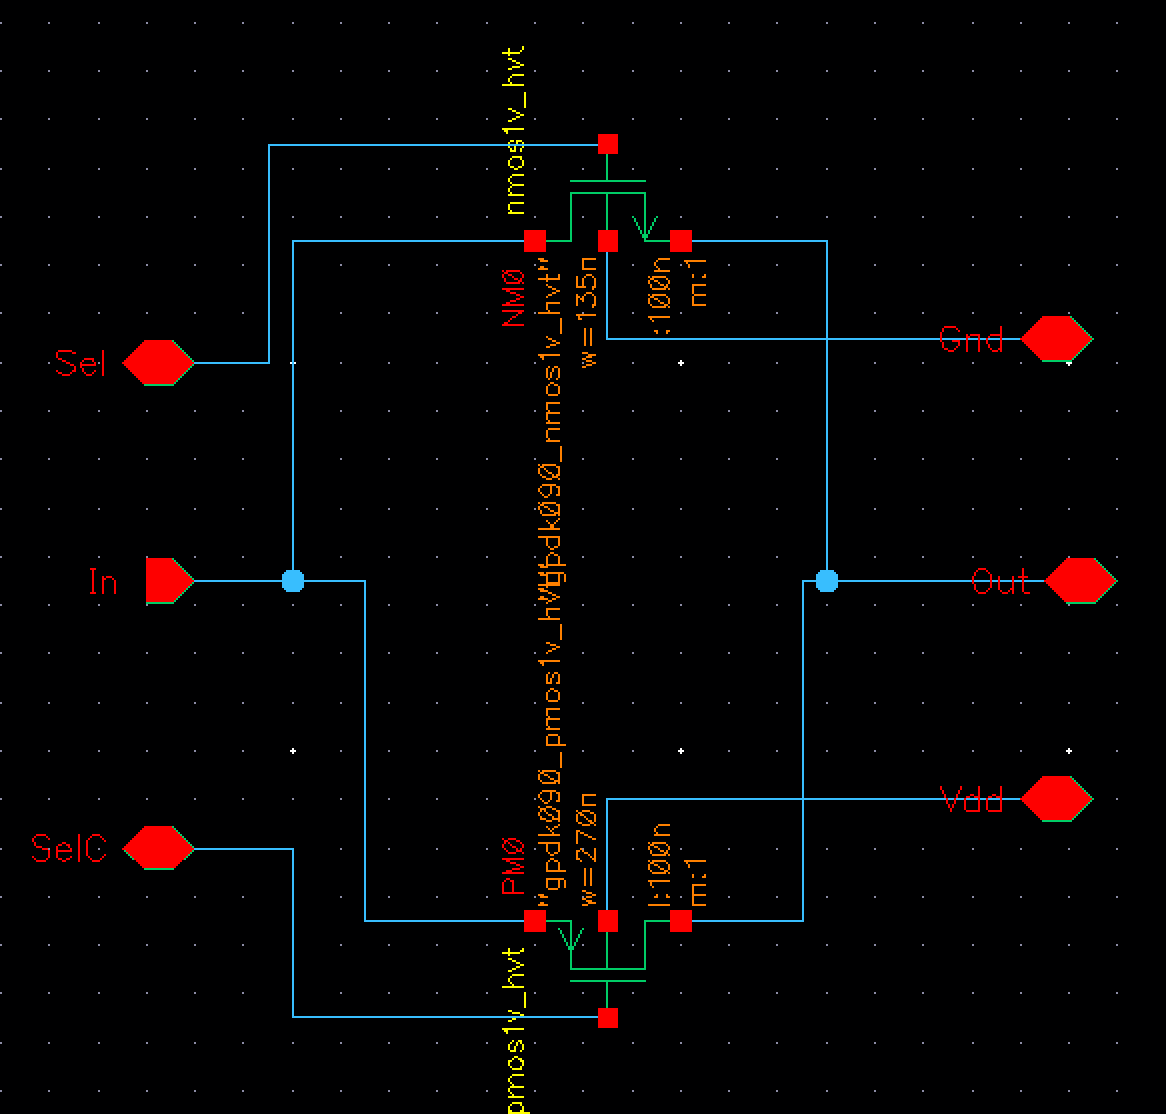
\includegraphics[scale=0.4]{tgate.png} \\
	 \newline \newline \newline \newline \newline \newline \newline \newline
	Shifter:\\
 	 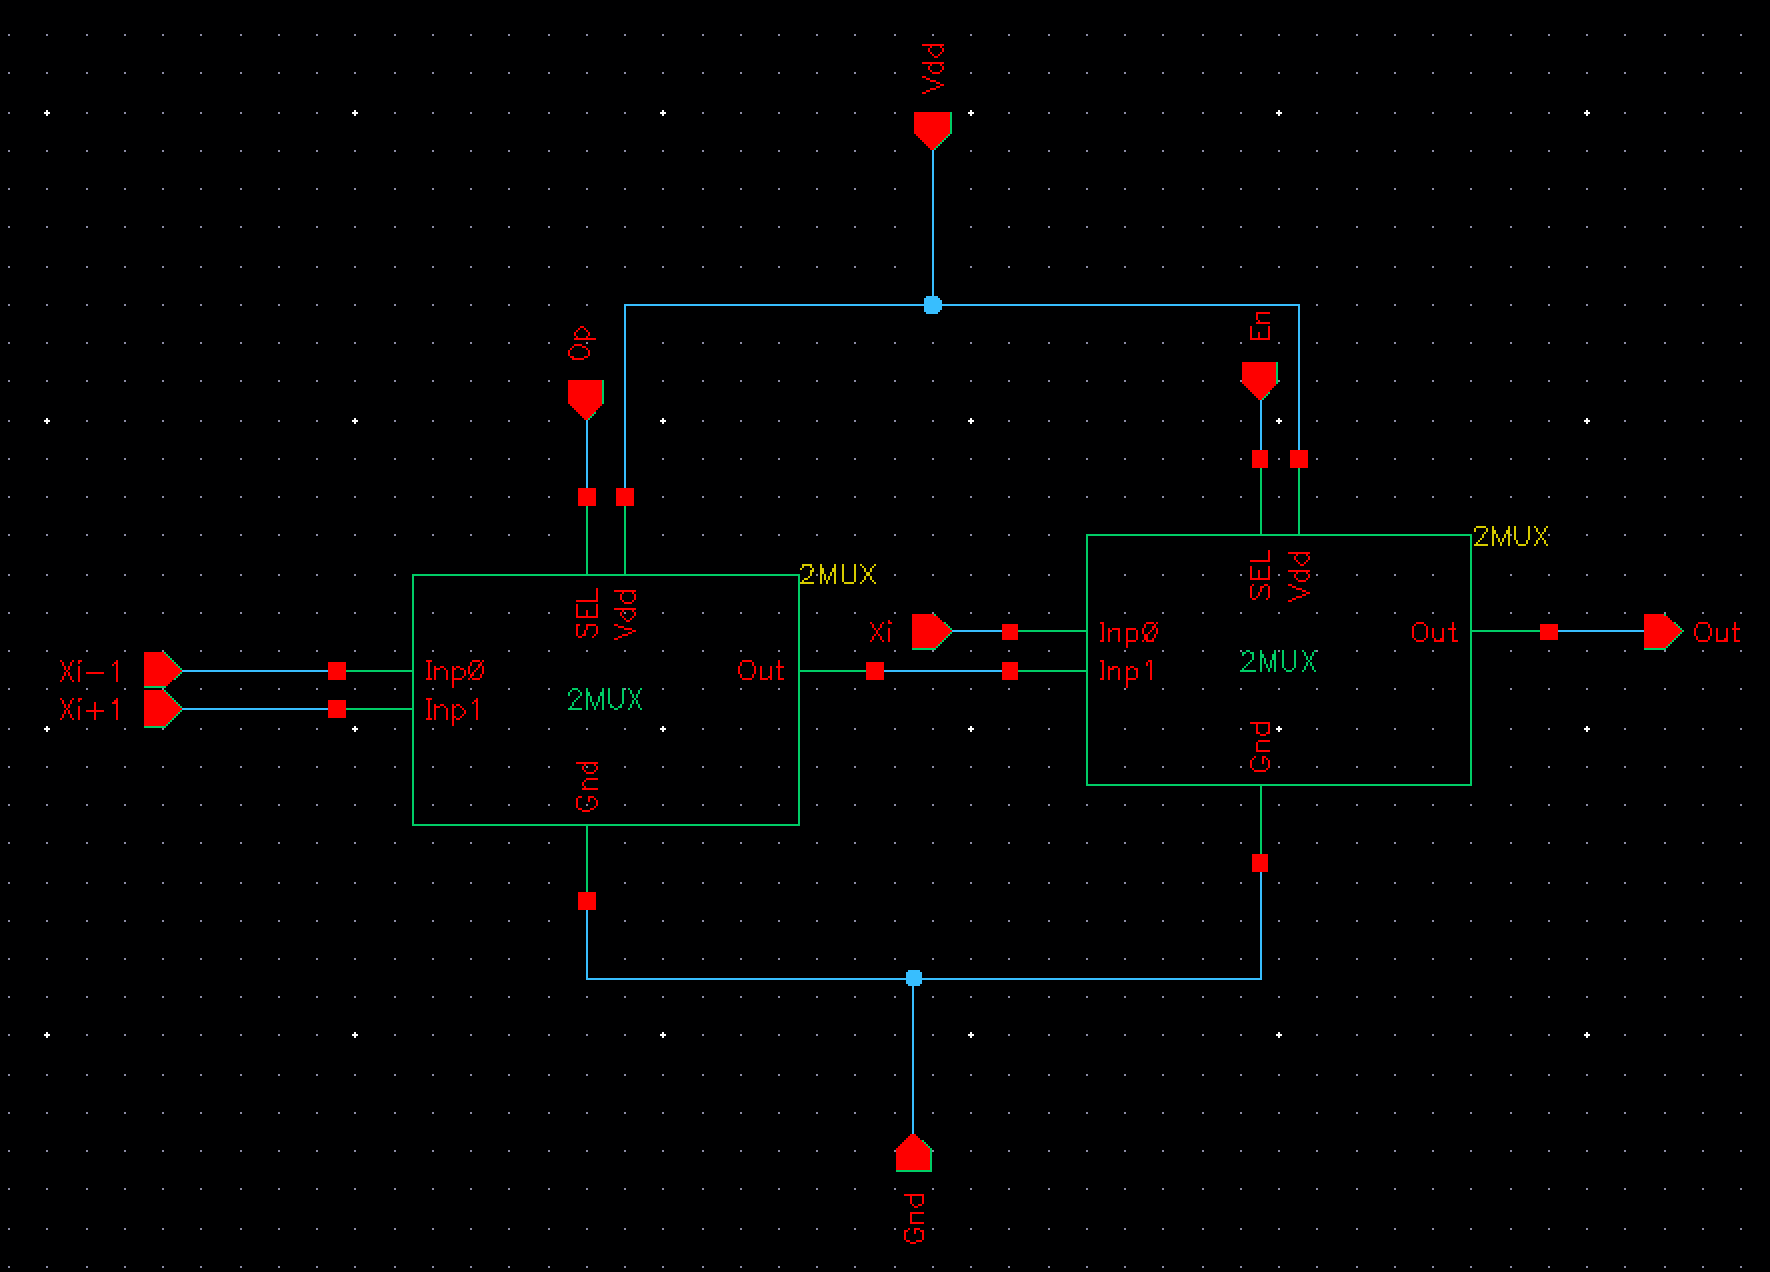
\includegraphics[scale=0.3]{shift.png} \\
	 \newline \newline
	Partial Demux:\\
  	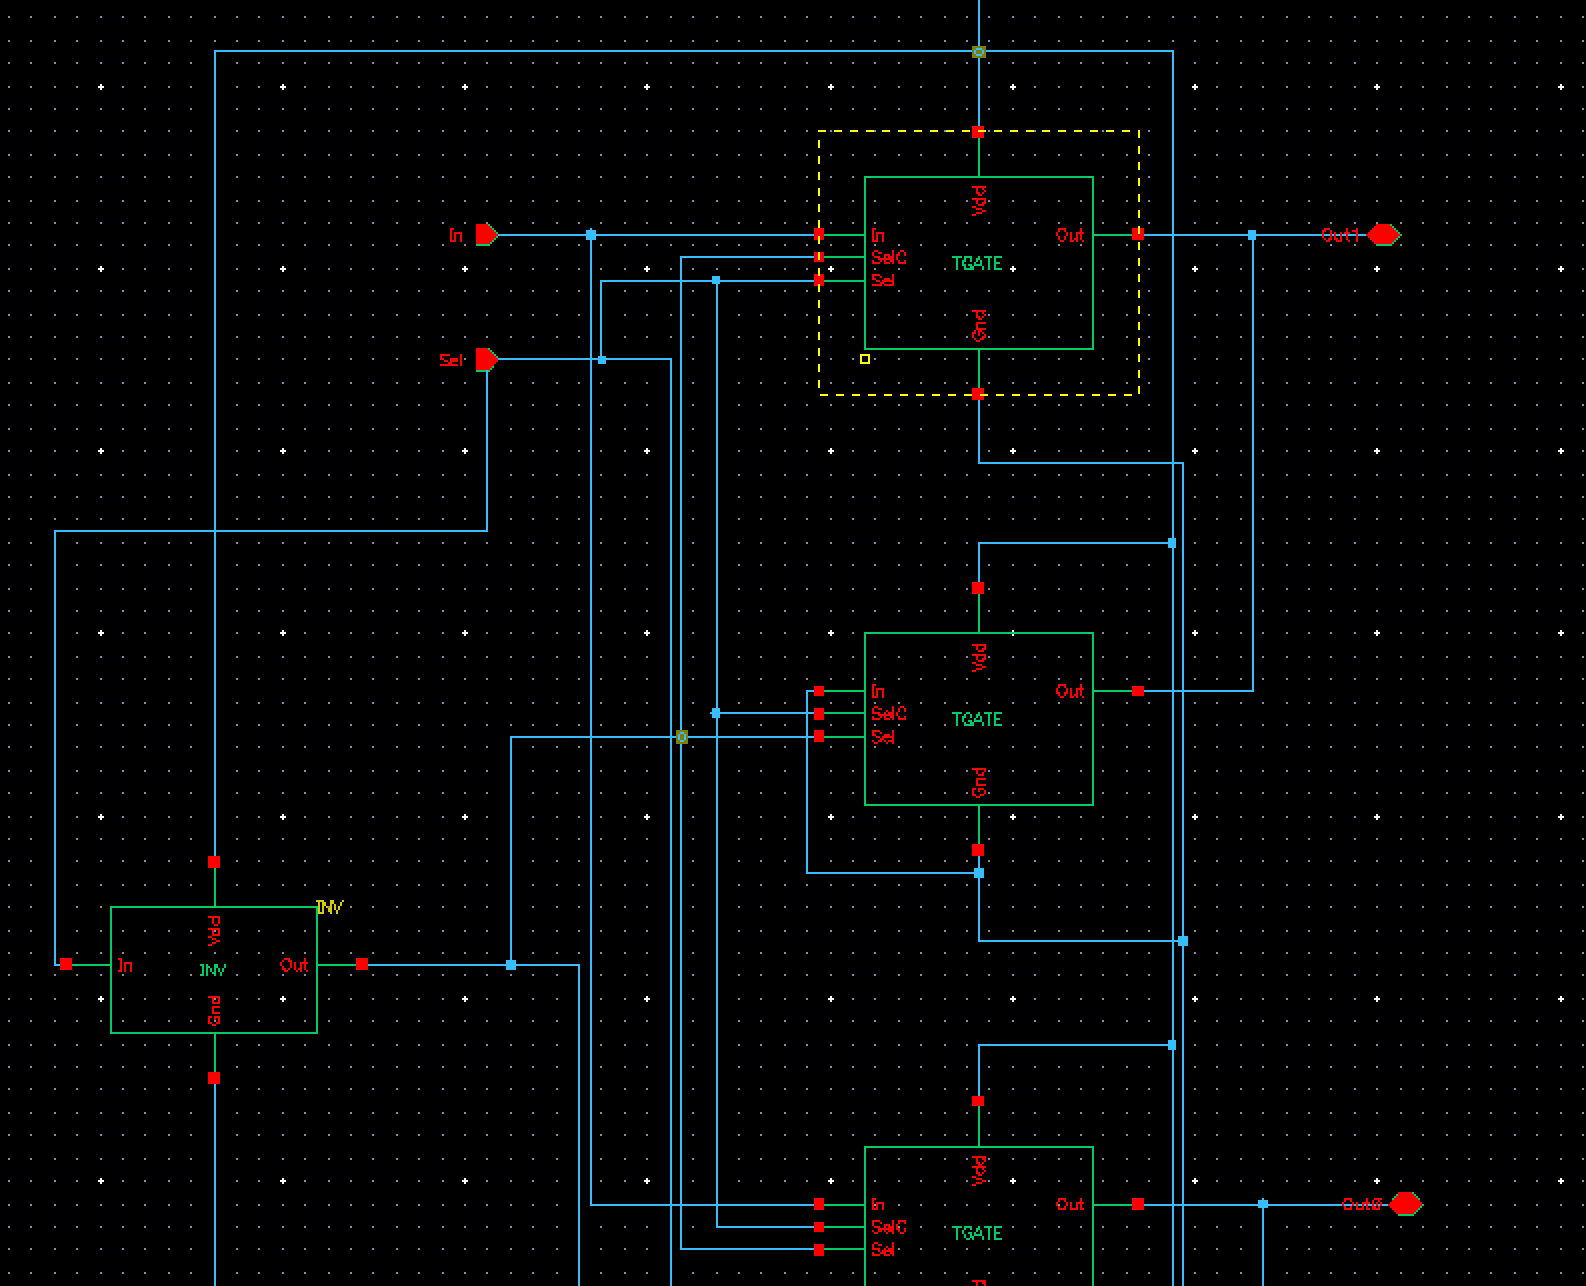
\includegraphics[scale=0.4]{demuxpart.png} \\
	\newline \newline
	A final large 8-input MUX was then used to serve as the final channel to the ultimate output 
	bit for the slice. Though each OpCode is 4 bits in length, we managed to come up with an 
	interesting mapping such that only the 3 least significant bits are used:
	\newline \newline
  	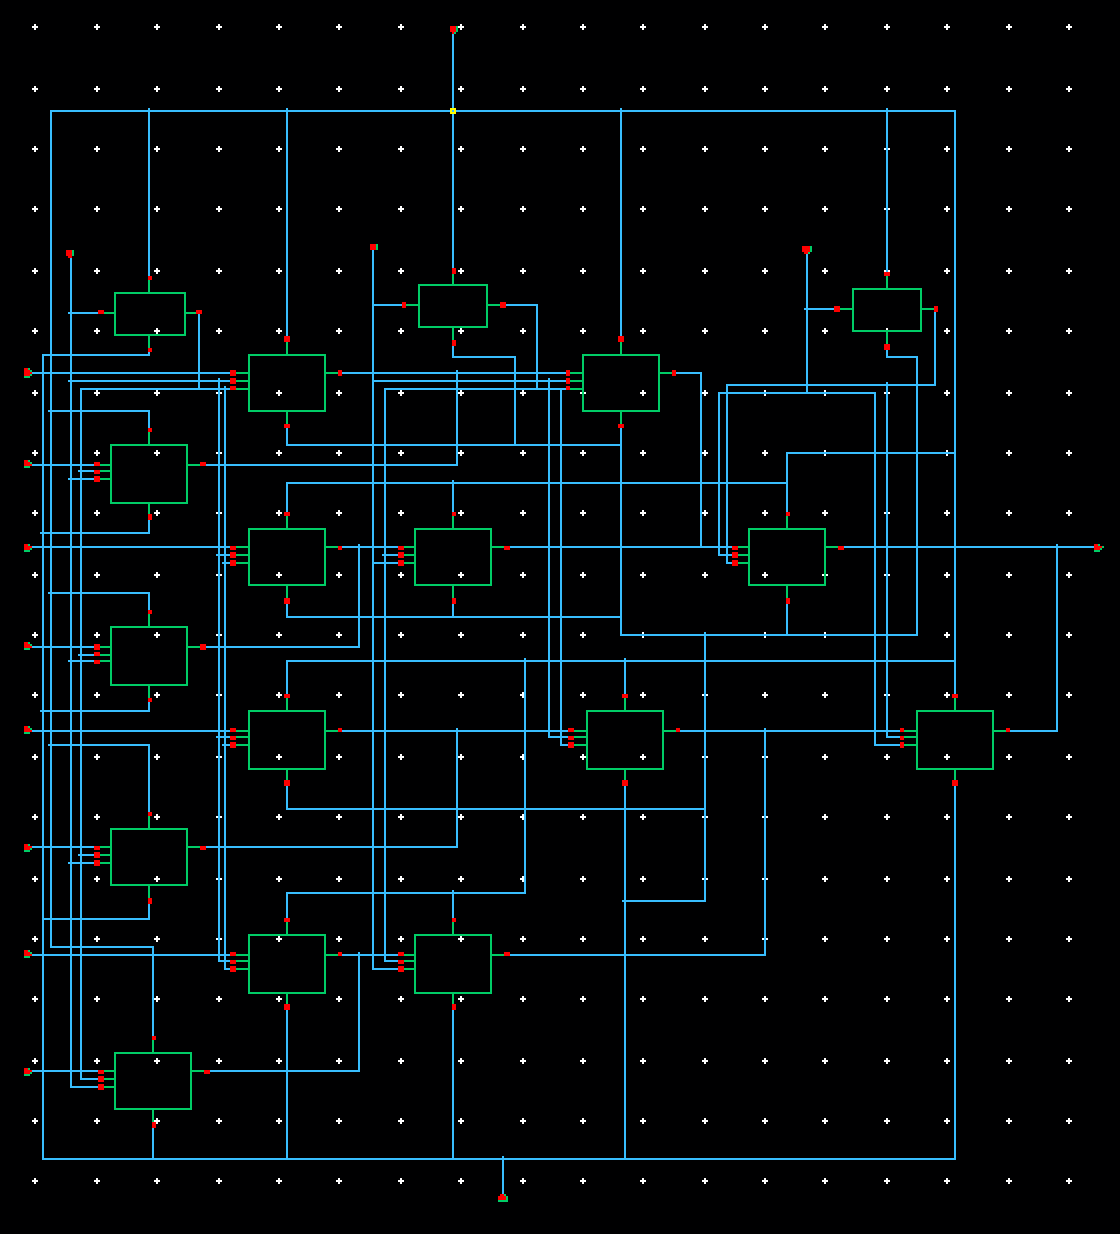
\includegraphics[scale=0.4]{8mux.png} \\
	\newline \newline
	\textbf{Adder Implementation:}
	\newline \newline
	We chose to go with a Carry Look-Ahead adder implementation using a combination of AND,
	OR, and XOR gates, as shown below:
	\newline \newline
 	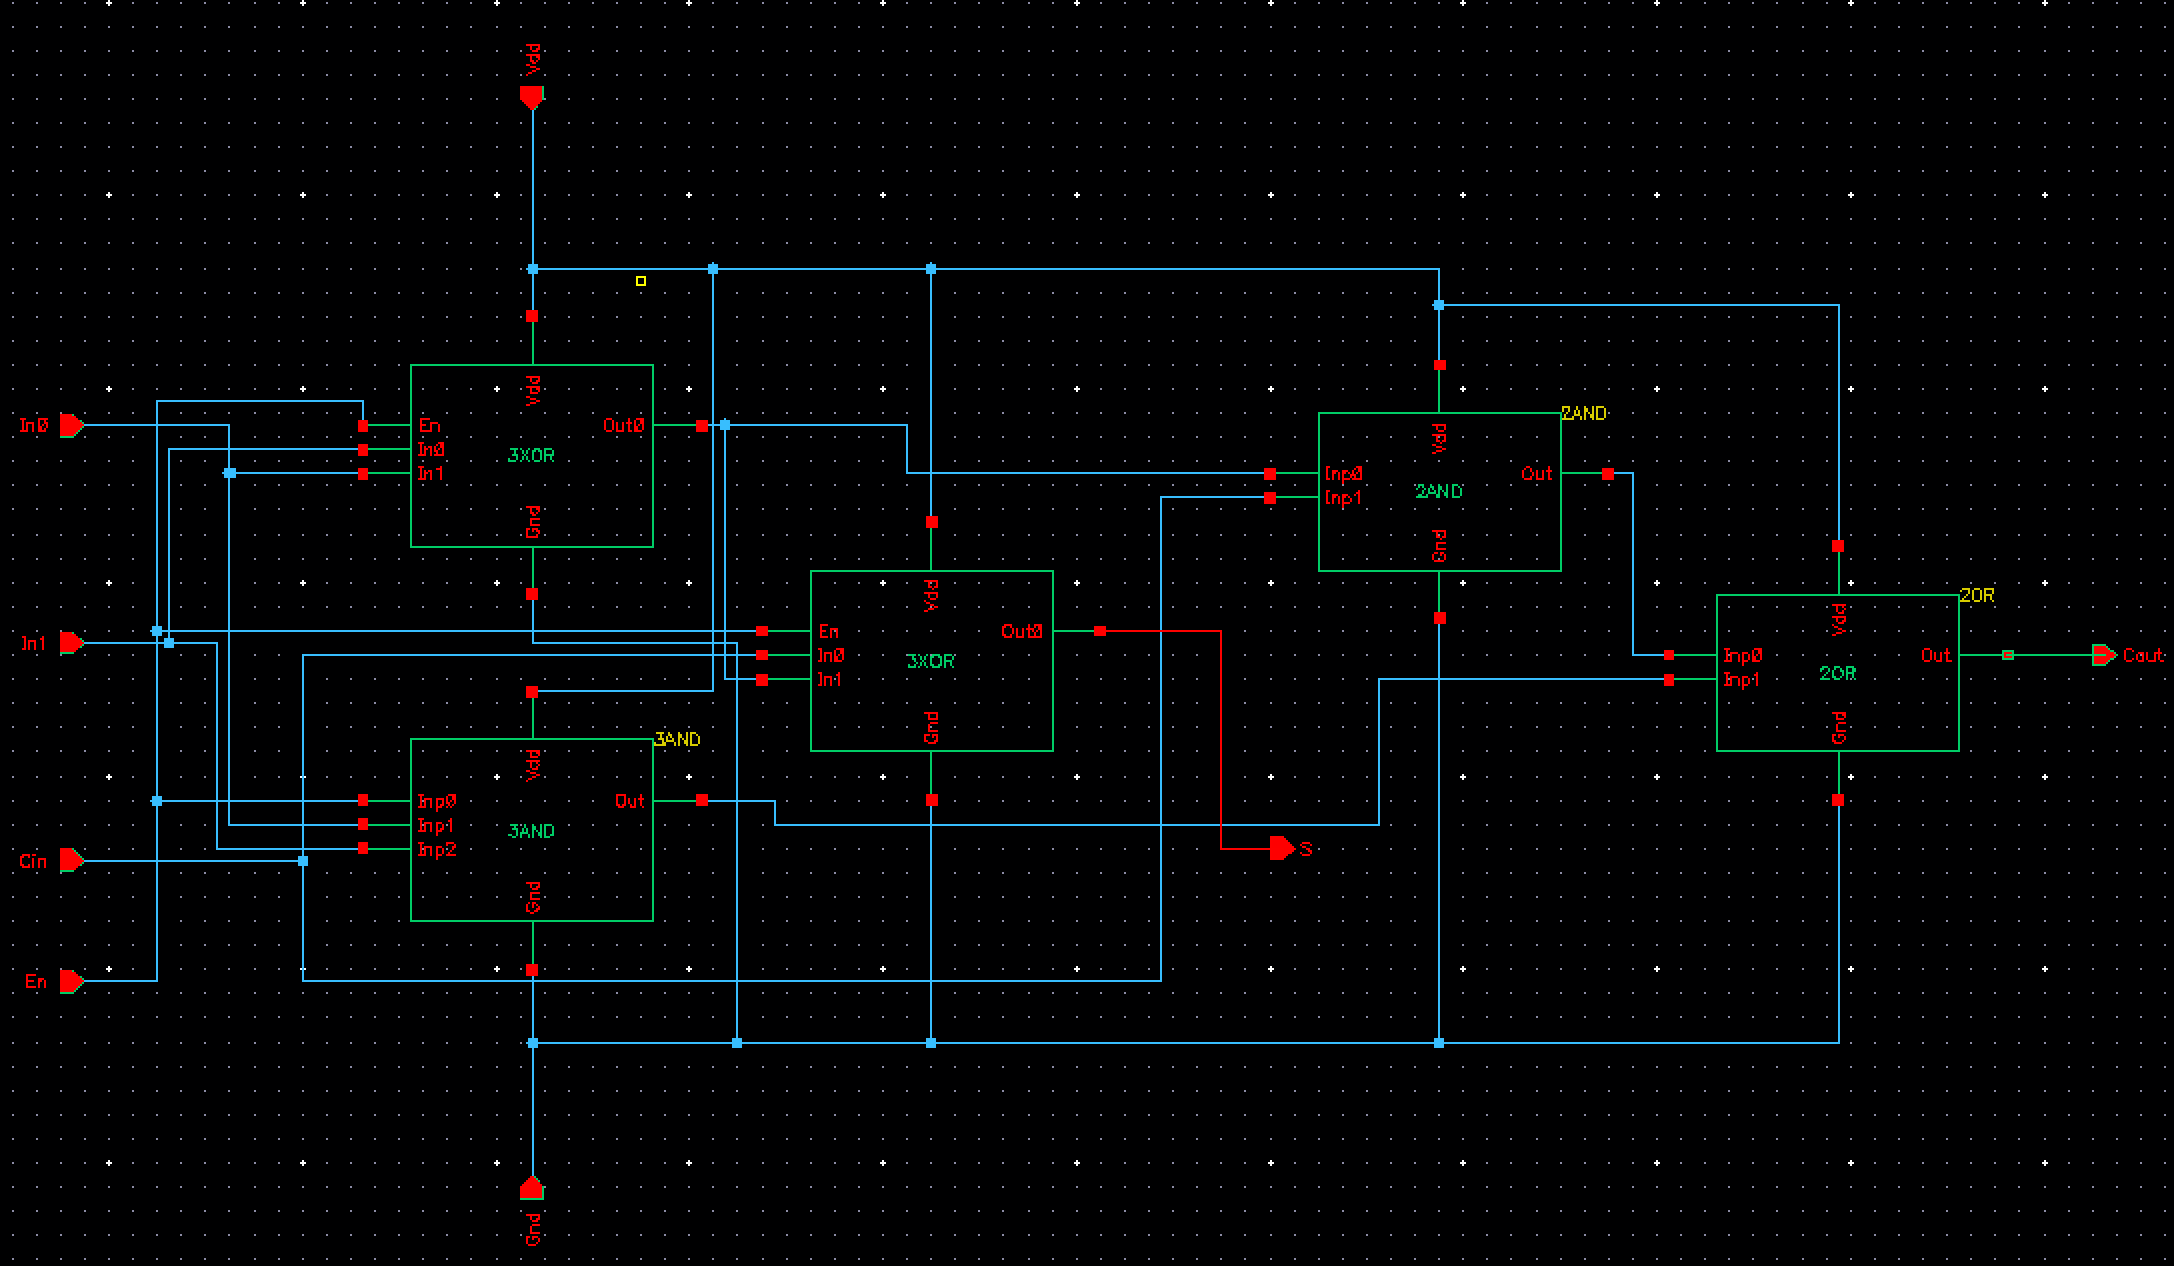
\includegraphics[scale=0.4]{add.png} \\
	\newline \newline
	The Look-Ahead implementation would allow for the parallel computation of the Carry-Out and
	Sum quantities, which would allow us to quickly send the carry-out number on the look-ahead
	bus for other bit slices to absorb. In this regard, we would be significantly reducing the delay
	of the adder module and a reasonable amount of power consumption as well. This minimization
	is further supported by the fact that the adder does not even activate unless the enable bit
	is activated (controlled via a combination of DEMUX gates). Future iterations of the project 
	may include changing this implementation, but for now the attempt seemed good enough to
	suffice.
	\newline \newline
	\textbf{Ending Remarks:}
	\newline \newline
	All components were tested individually for correct functionality before being incorporated 
	into other blocks of the circuit.
	\newline \newline
	
  	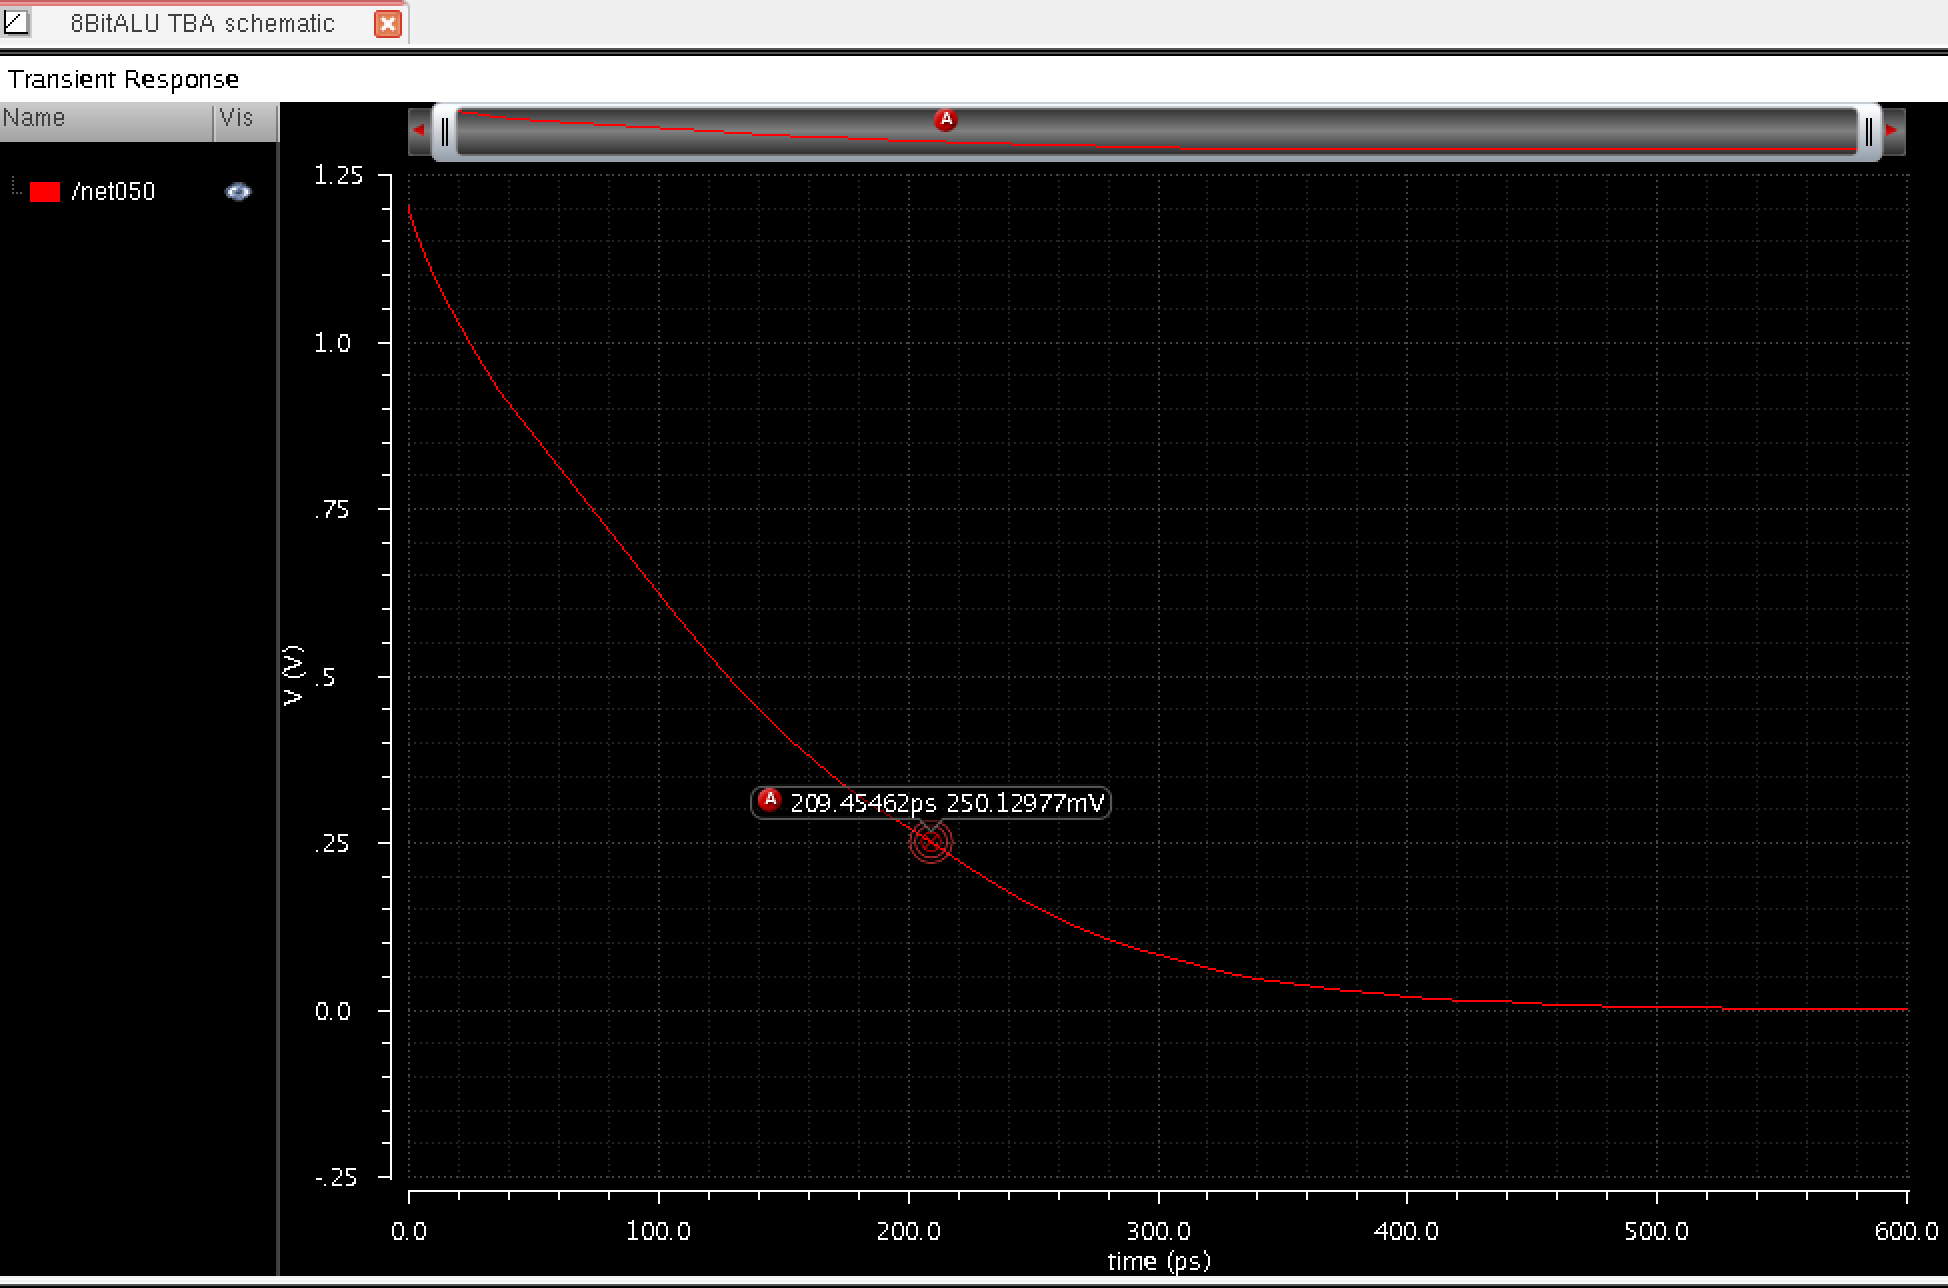
\includegraphics[scale=0.4]{AndDelay.png} \\
	\newline \newline
  	This demonstrates the delay from the Bitwise AND instruction in the ALU. While not the worst 
	delay path in the ALU, it does a resonable approximation of the work that must be done, since 
	it travels along the farthest path (besides adder instructions). The propagation delay
	here is about 209 ps.
	\newline \newline
	After trying a variety of OpCodes, we found that the slice worked as far as functionality 
	is concerned. For this stage of the project, this was a reasonable testament of our progress
	and hard work.
	\newline \newline
	\textbf{Next Steps:}
	\newline \newline
	In addition to doing the full transistor layout, we may also decide to revise our designs. Since
	our circuit is modular, this would be reasonably simple to do. We have also not looked into
	one operation in particular - loading X into memory. For this reason, one particular input pin 
	of the 8-input MUX has been left dangling. It will be connected to the loaded bit value of
	X after this block has been implemented. 
  \section{}
	
  \textbf{Layouts}
  \newline \newline
  The layouts werw a semi-complicated beast. Once we got the hang of creating the module layouts
  and have them be in the larger circuits, the process got easier. However, every time an LVS failed
  somewhere lower down, each higher circuit needed to be redone to accomadate for said changes.
  \newline \newline
  The master layout:
  \newline \newline
  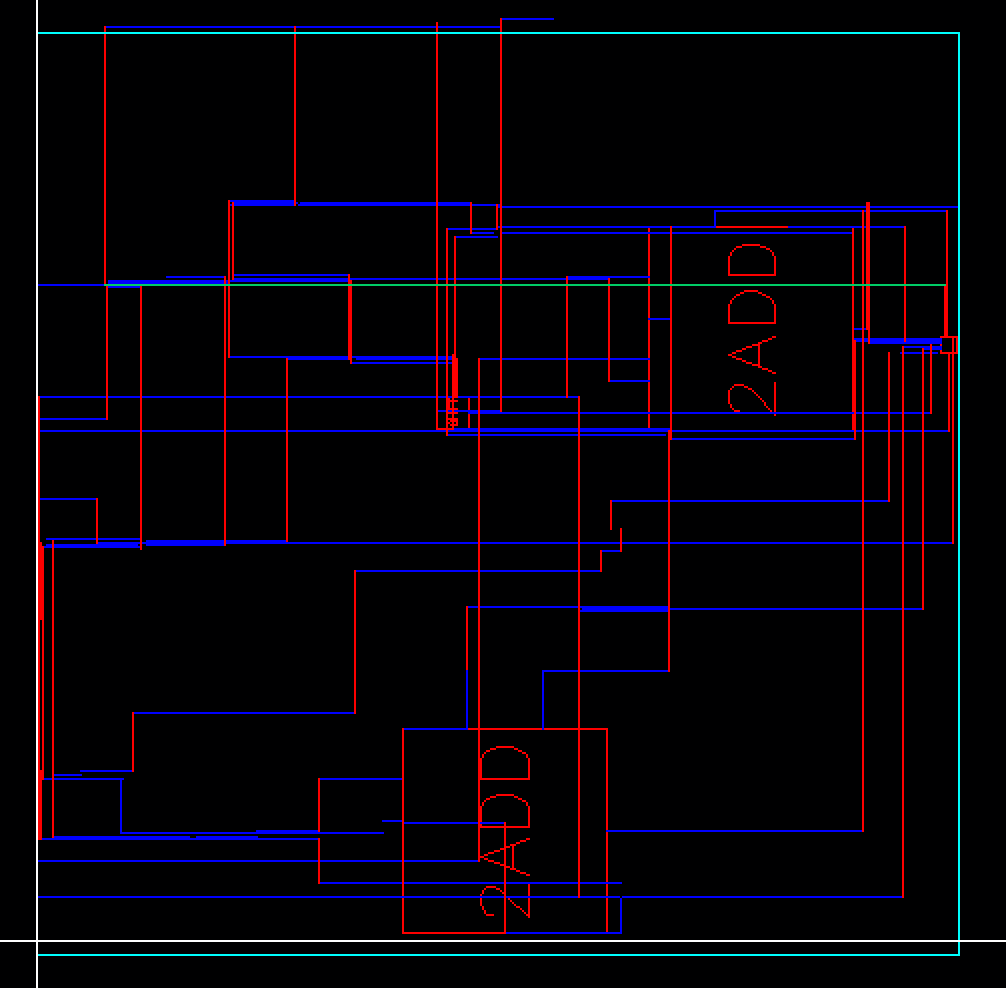
\includegraphics[scale=0.5]{masterlayout.png} \\
  \newline \newline
  As you can see, the adder is easily the largest module in the layout. 
  \newline \newline
  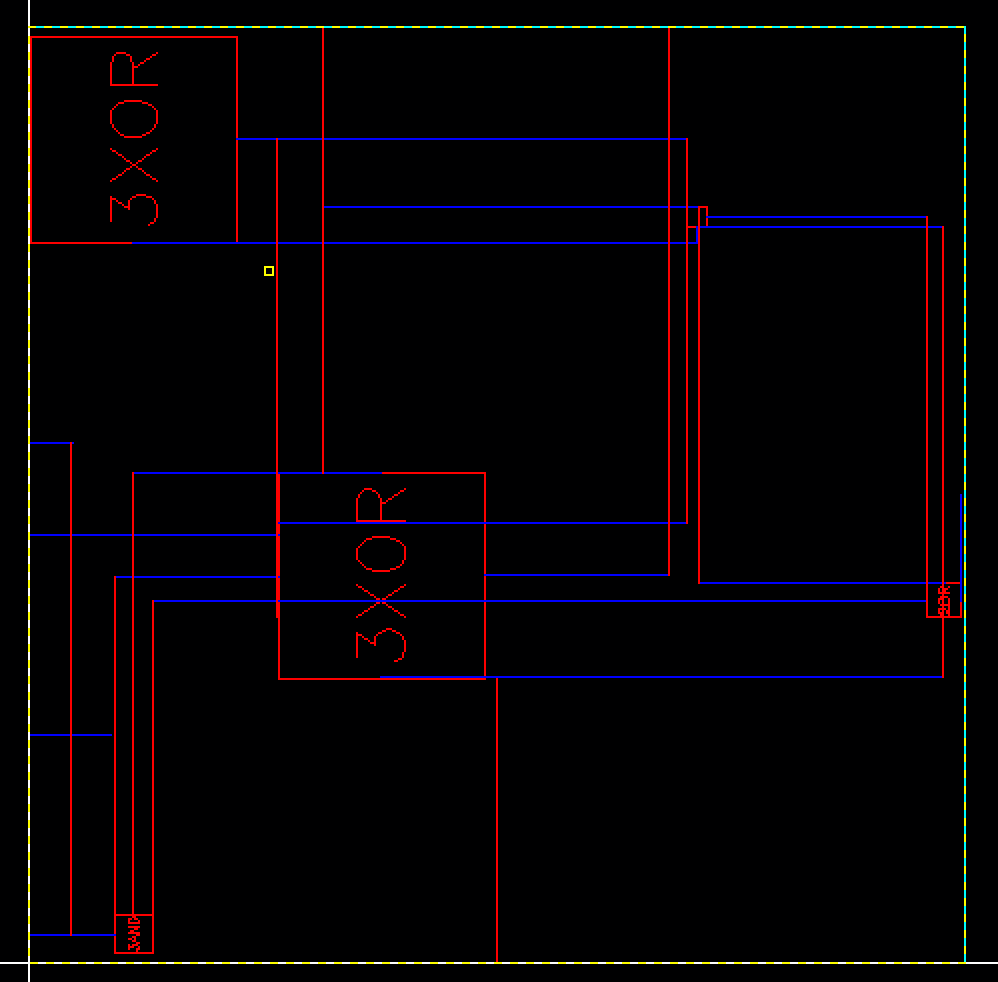
\includegraphics[scale=0.5]{adderlayout.png} \\
  \newline \newline
  Which, in turn, has XOR's and AND's. Obviously, the XOR is bigger than the AND.
  \newline \newline
  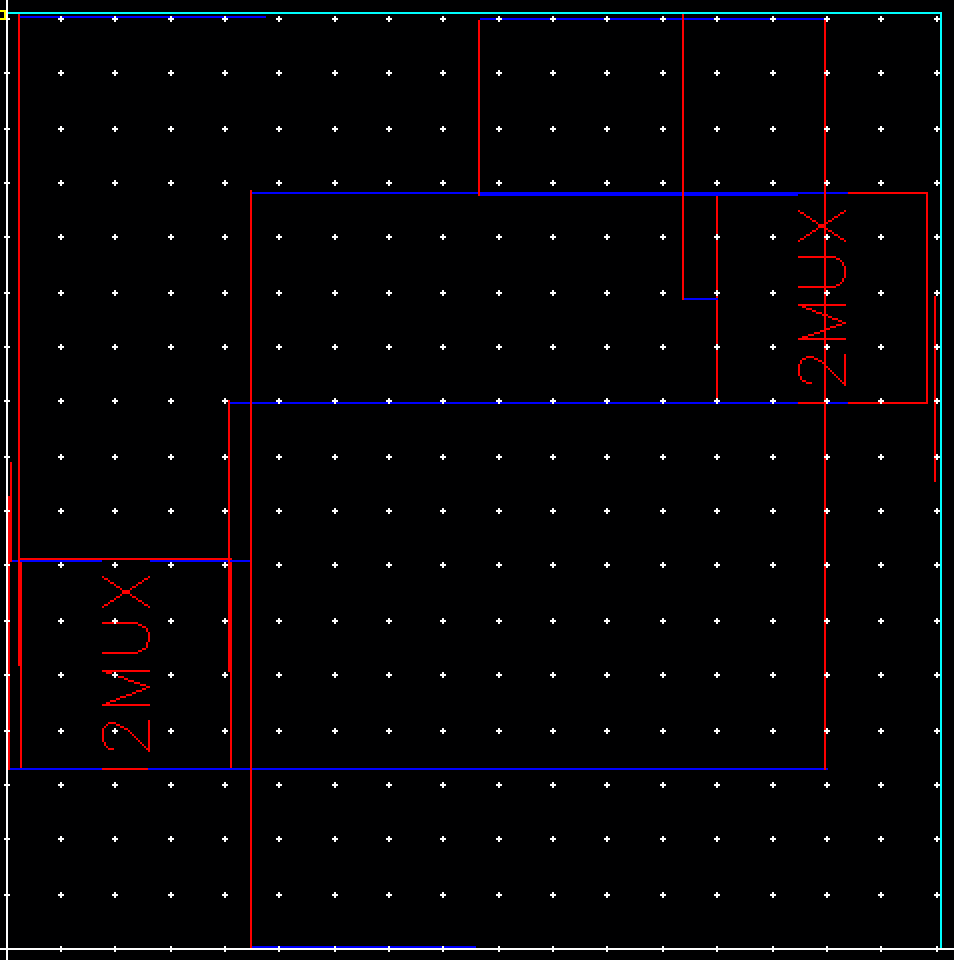
\includegraphics[scale=0.5]{shiftlayout.png} \\
  \newline \newline
  The shifter, made of 2MUX's is relatively straightforward when moving from schematic to layout.
  \newline \newline
  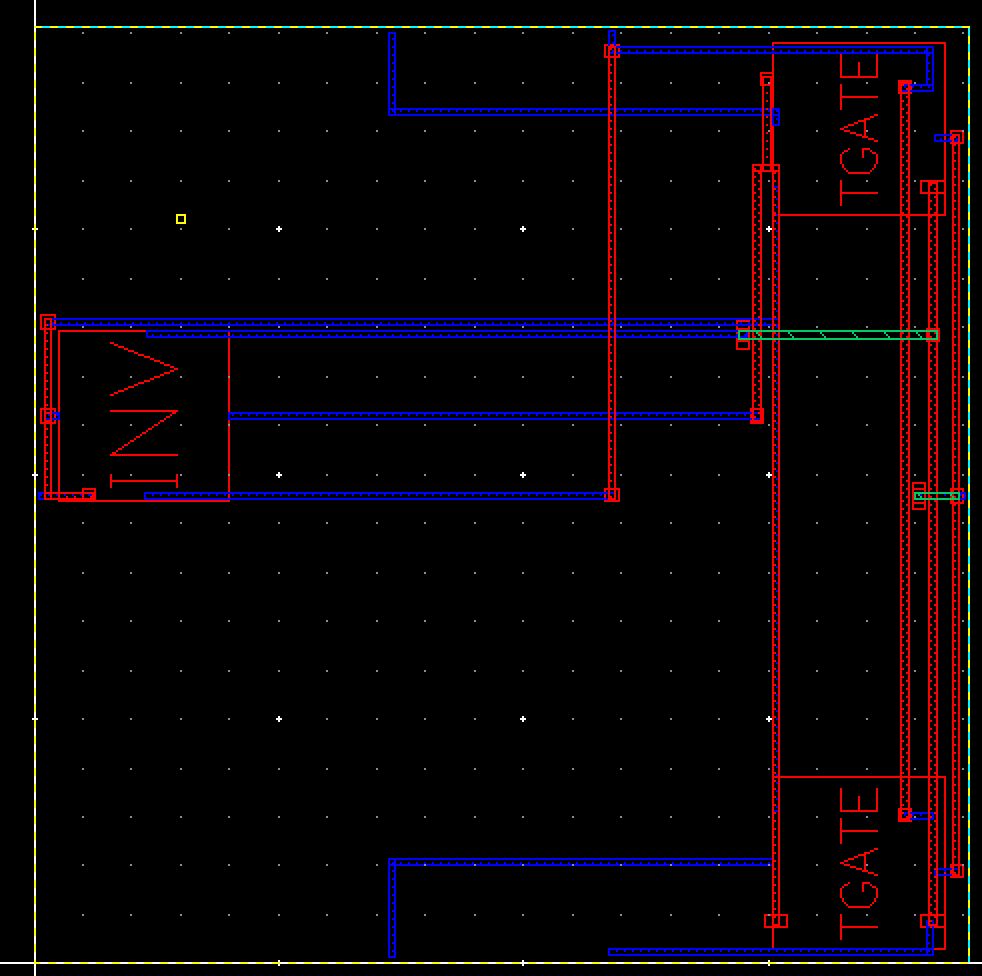
\includegraphics[scale=0.5]{muxlayout.png} \\
  \newline \newline
  And the mux has 2TGATE's and an INVERTER. Simple, straightforward compared to the master.
  \newline \newline
  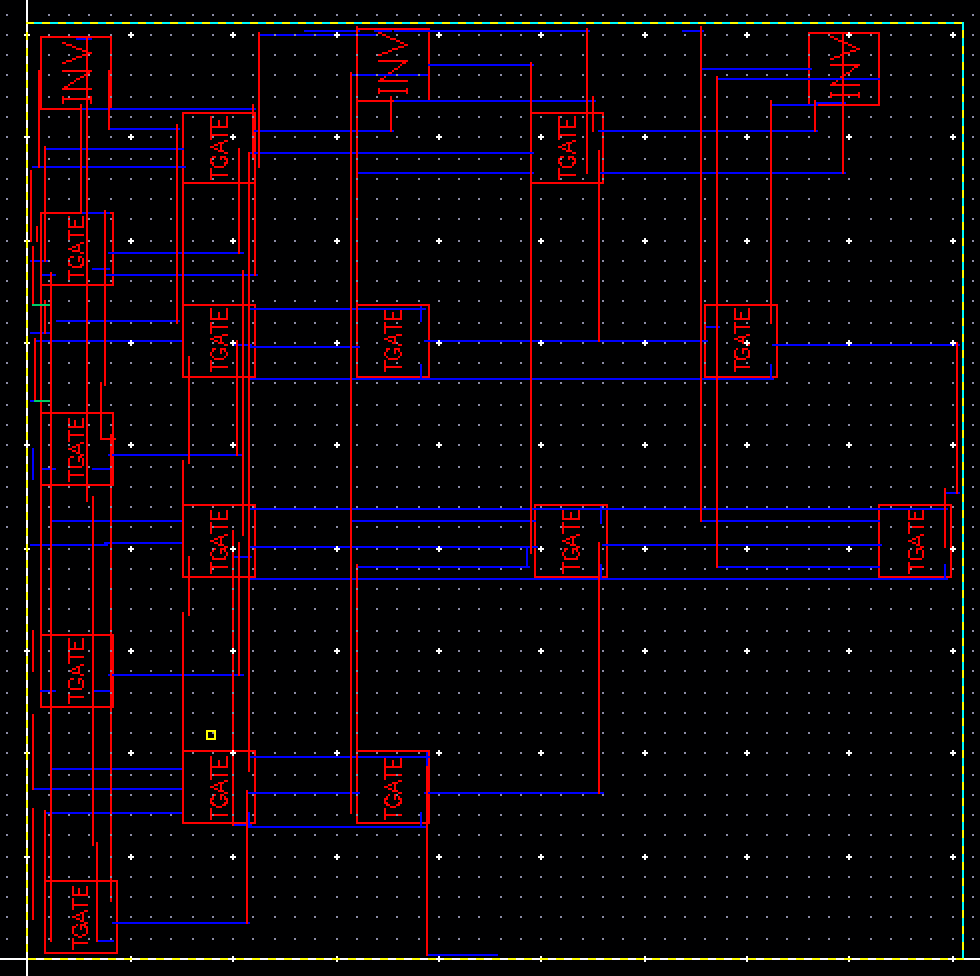
\includegraphics[scale=0.5]{8muxlayout.png} \\
  \newline \newline
  The 8 mux wasn't straightforward, however. But it's layout was repetitive, which in its very nature 
  made mistakes easier to catch.
  \newline \newline
  All in all, the only headache came when, for no reason, the automatic routing would simply not the
  Vdd and Gnd connections, or wire the body of the transistors to the wrong placed. 
  \newline \newline
	\textbf{A Look at the Adder Delay}
  \newline \newline
  For the adder, as mentioned previously we used the carry-lookahead methodology to implement it.
  From there, we took two measurements: one of the propagation delay on the ouput, and the other on
  the propagation delay of the carry-out. The following graphics demonstrate the delays:
  \newline \newline
  \newline \newline
  Delay of sum on the adder:
  \newline \newline
  \newline \newline
  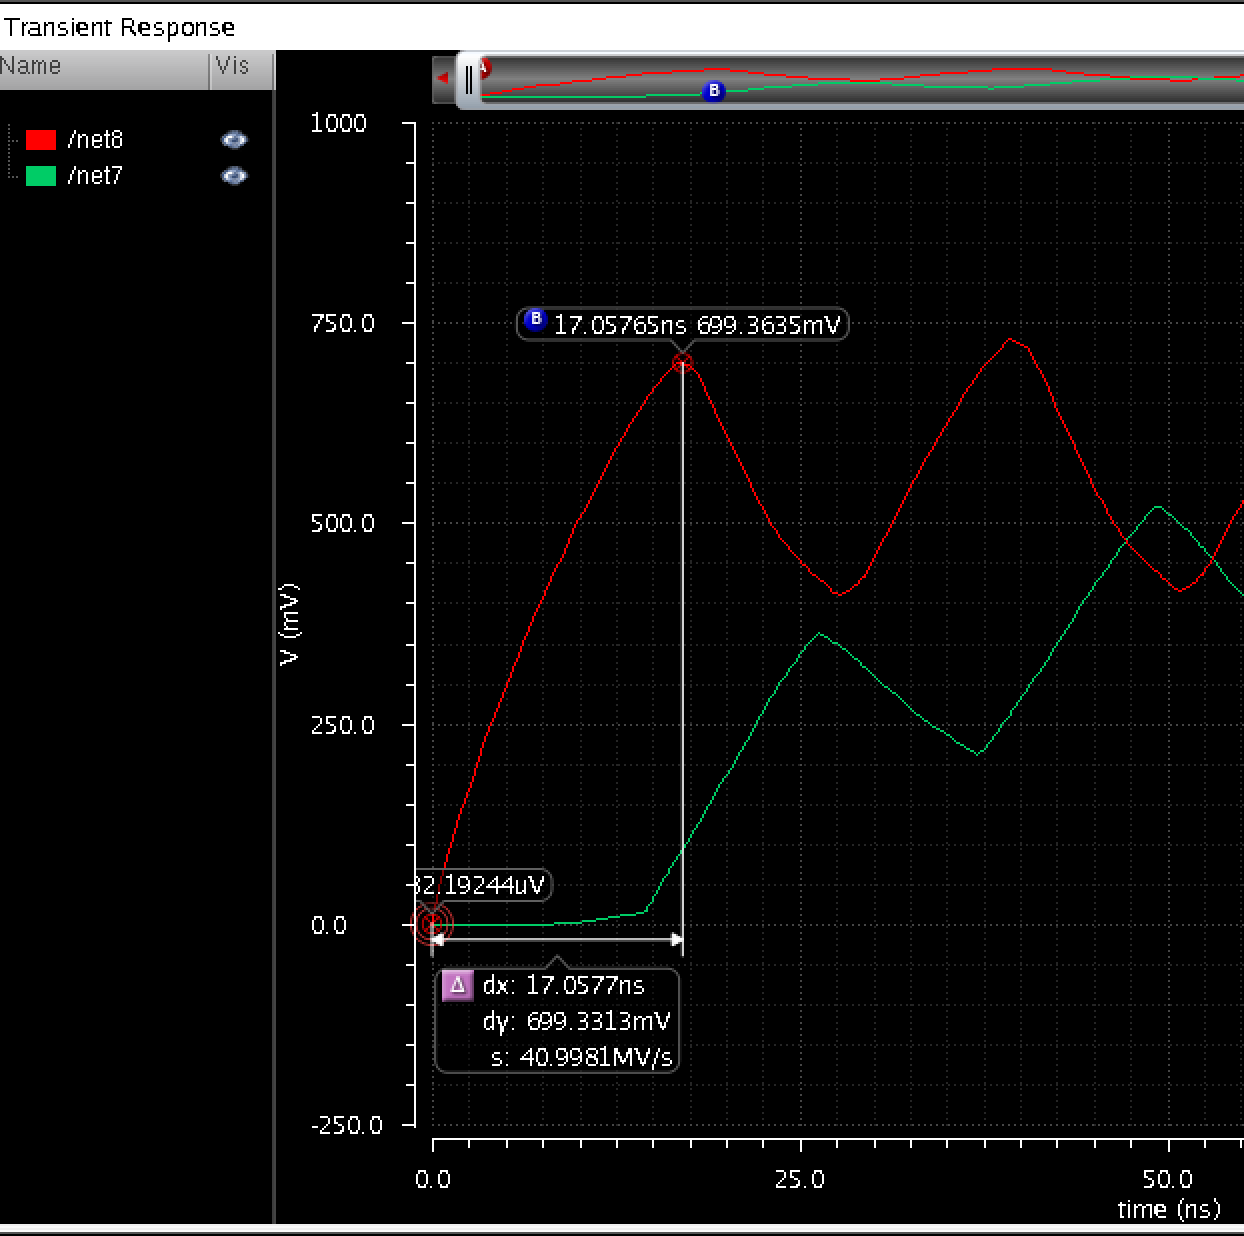
\includegraphics[scale=0.4]{delaysum.png} \\
  \newline \newline
  \newline \newline
  \newline \newline
  \newline \newline
  Delay of cout on the adder:
  \newline
  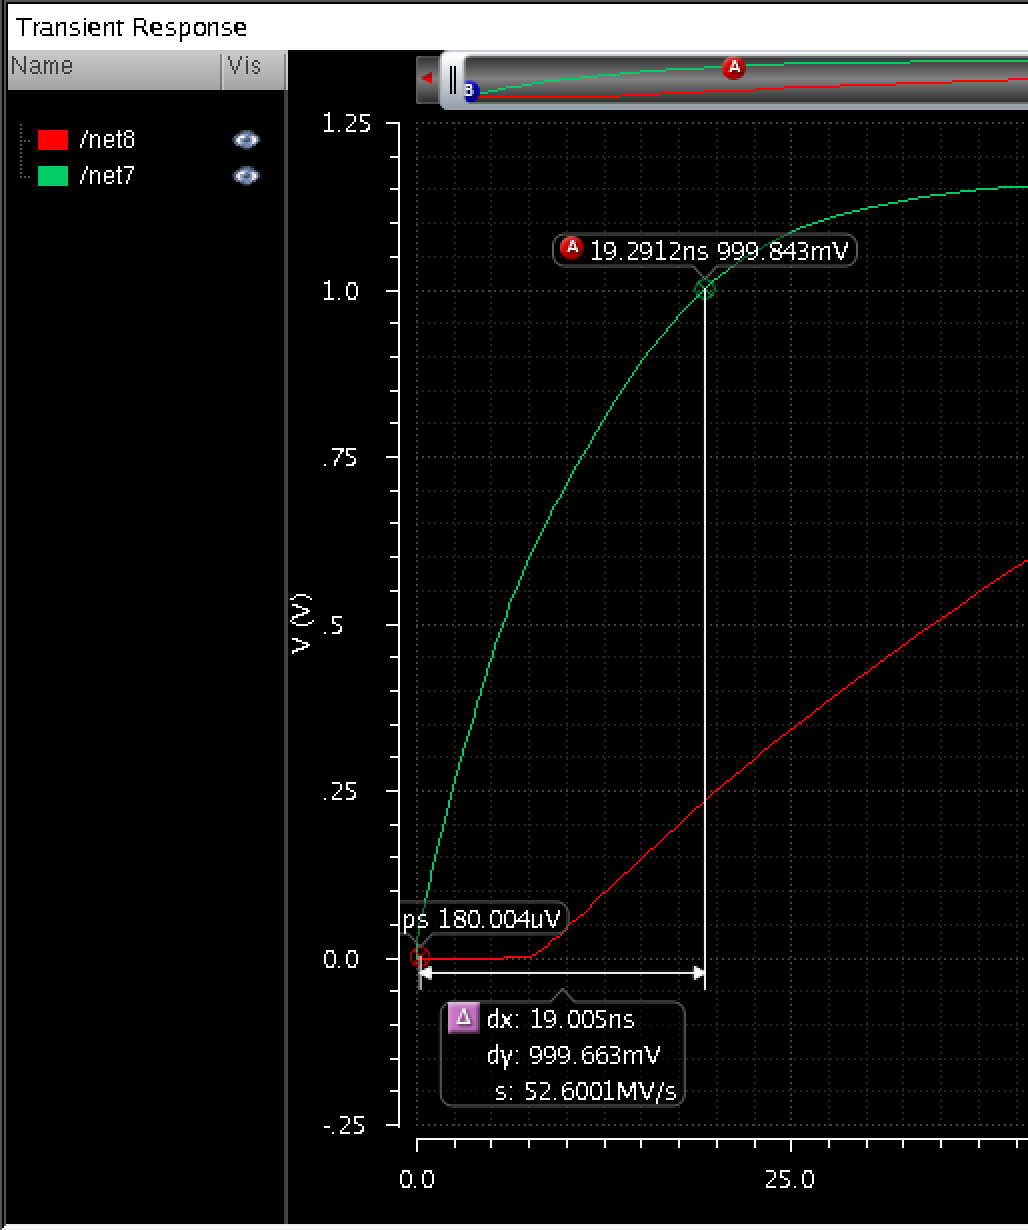
\includegraphics[scale=0.4]{delaycout.png} \\
  \newline \newline
  As the graphs portray, the sum takes about 17.057 ns and the cout takes about 19.29 ns. That's
  not good. but we will fix that by doing better transistors sizing to pass the constants necessary
  for the cout to come faster. Currently, they are all of uniform size, which is not ideal and will
  be fixed in a timely manner.
  \newline \newline
	\textbf{Energy Consumption}
  \newline \newline
  The dynamic energy consumption is a factor of the amount of swiching done by the transistors due
  the work being done. Using the Calculator in Cadence, the graphic below demonstrates that energy 
  consumption (and power, for that matter).
  \newline \newline
  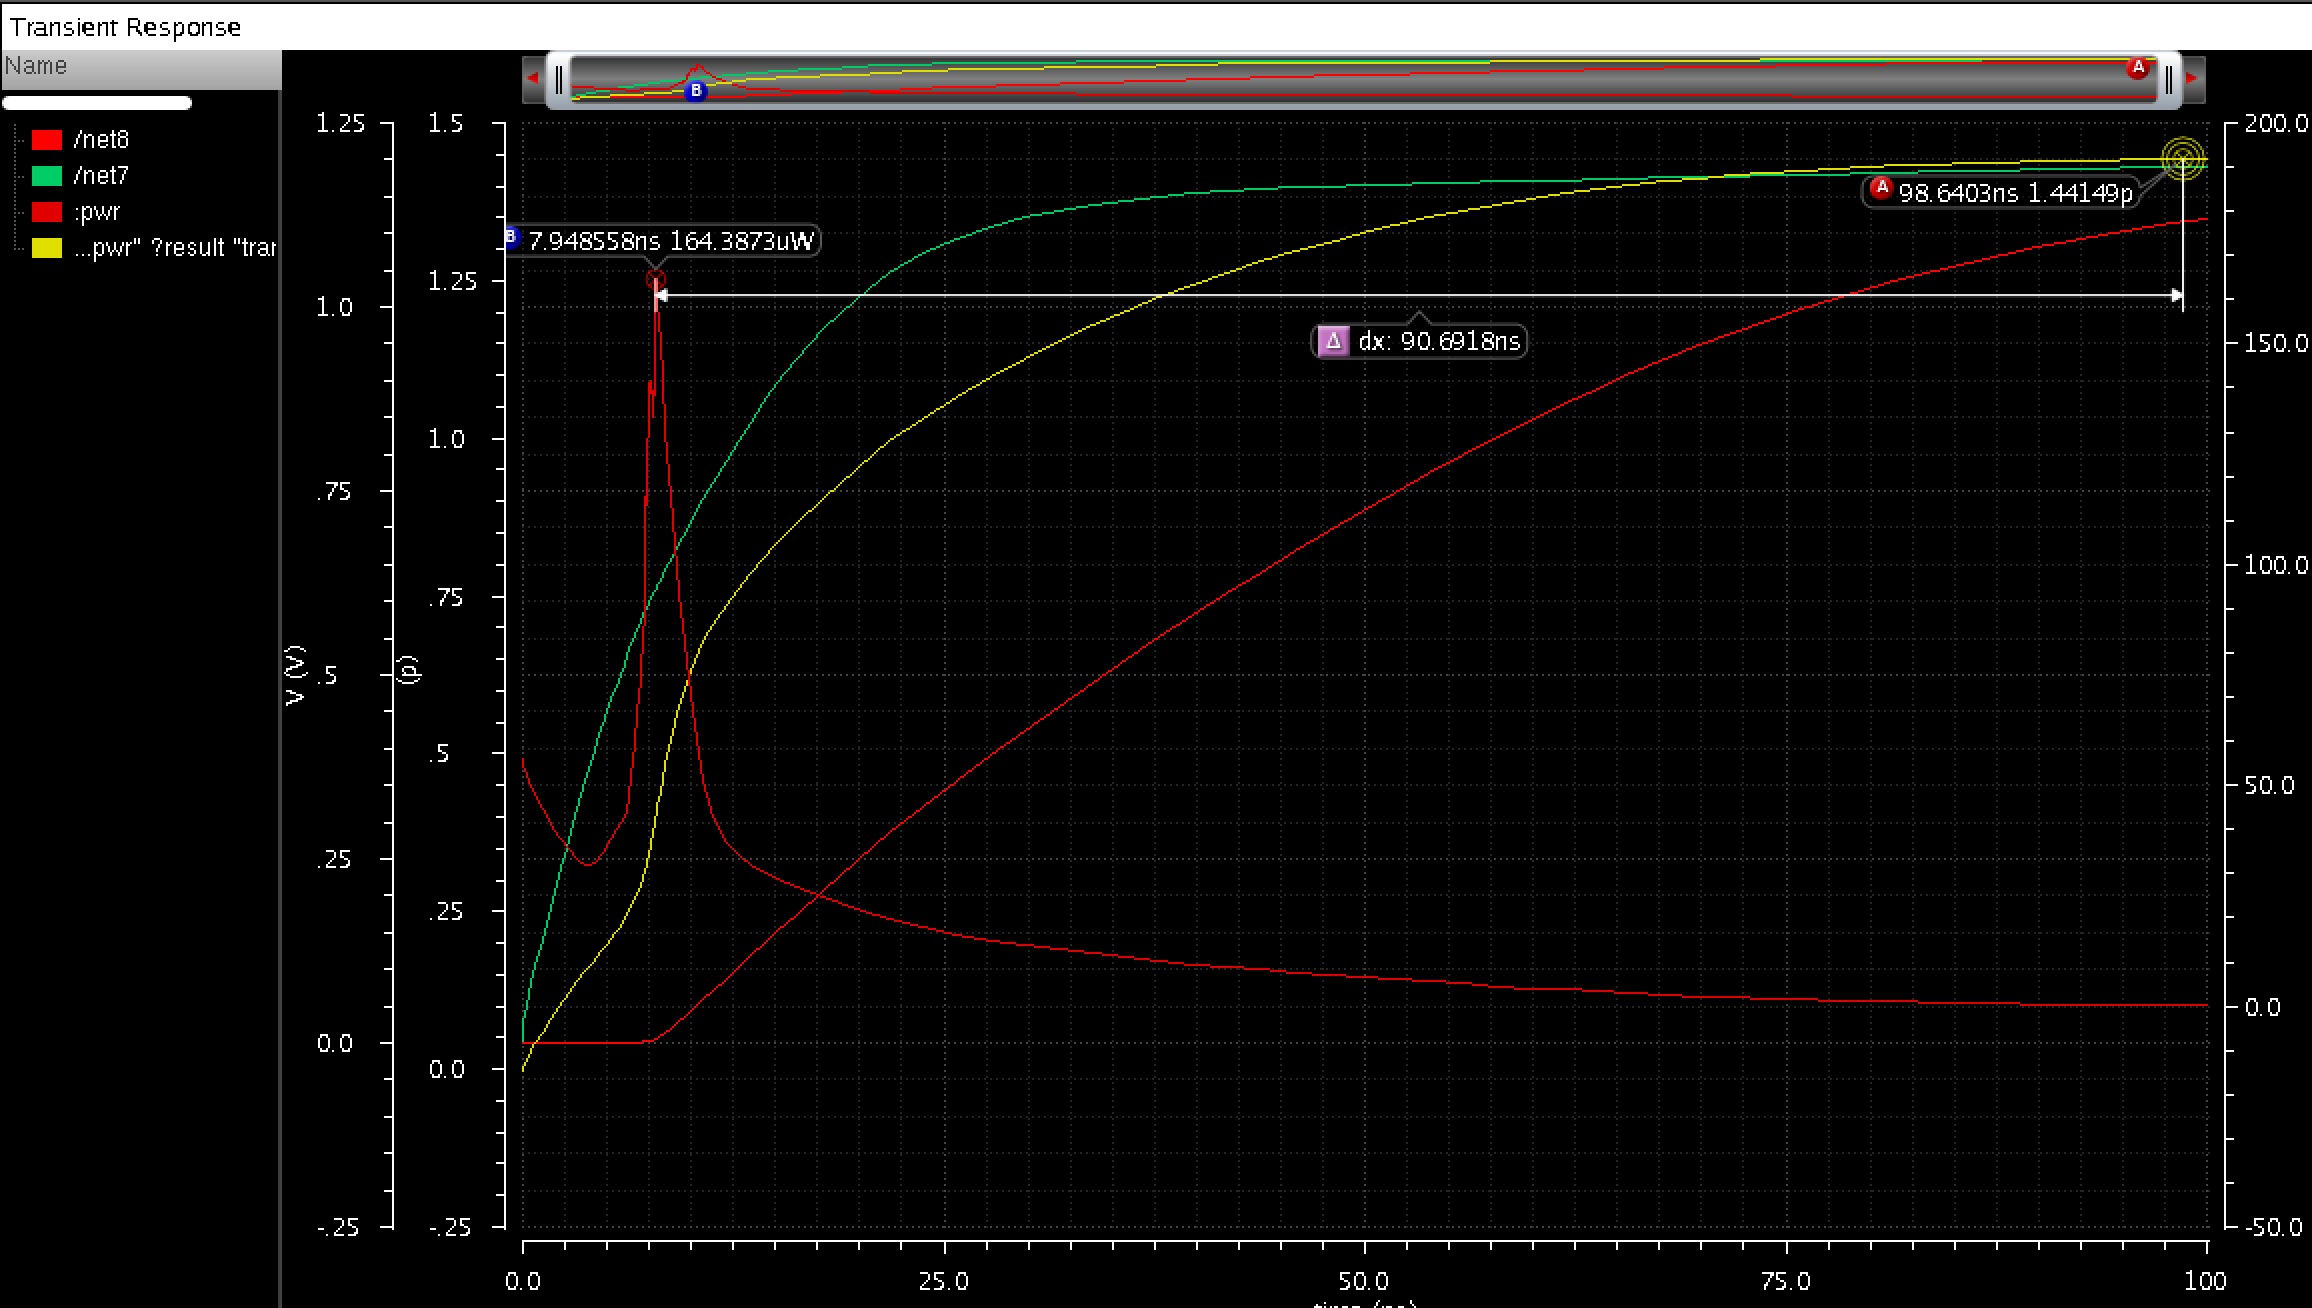
\includegraphics[scale=0.4]{energy.png} \\
  \newline \newline
  The peak power output was about 164 $\mu$ W, and the dynamic energy consumption is about 1.44 pJ.
  This is represtentative of a majority of the paths in our circuit. If anything, only the subtract
  instruction will incur a slightly larger energy consumption. Other than that, the energy is upper-bounded
  by this, since use of the adder in the ALU is the most expensive procedure.
    
  


\end {document}


